\documentclass[letterpaper]{article}
%\documentclass[a5paper]{article}

%% Language and font encodings
\usepackage[english]{babel}
\usepackage[utf8x]{inputenc}
\usepackage[T1]{fontenc}


%% Sets page size and margins
\usepackage[letterpaper,top=.75in,bottom=1in,left=1in,right=1in,marginparwidth=1.75cm]{geometry}
%\usepackage[a5paper,top=1cm,bottom=1cm,left=1cm,right=1.5cm,marginparwidth=1.75cm]{geometry}

\usepackage{graphicx}
%\graphicspath{../images}	  %%where to look for images

%% Useful packages
\usepackage{amssymb, amsmath, amsthm} 
%\usepackage{graphicx}  %%this is currently enabled in the default document, so it is commented out here. 
\usepackage{calrsfs}
\usepackage{braket}
\usepackage{mathtools}
\usepackage{lipsum}
\usepackage{tikz}
\usetikzlibrary{cd}
\usepackage{verbatim}
%\usepackage{ntheorem}% for theorem-like environments
\usepackage{mdframed}%can make highlighted boxes of text
%Use case: https://tex.stackexchange.com/questions/46828/how-to-highlight-important-parts-with-a-gray-background
\usepackage{wrapfig}
\usepackage{centernot}
\usepackage{subcaption}%\begin{subfigure}{0.5\textwidth}
\usepackage{pgfplots}
\pgfplotsset{compat=1.13}
\usepackage[colorinlistoftodos]{todonotes}
\usepackage[colorlinks=true, allcolors=blue]{hyperref}
\usepackage{xfrac}					%to make slanted fractions \sfrac{numerator}{denominator}
\usepackage{enumitem}            
    %syntax: \begin{enumerate}[label=(\alph*)]
    %possible arguments: f \alph*, \Alph*, \arabic*, \roman* and \Roman*
\usetikzlibrary{arrows,shapes.geometric,fit}

\DeclareMathAlphabet{\pazocal}{OMS}{zplm}{m}{n}
%% Use \pazocal{letter} to typeset a letter in the other kind 
%%  of math calligraphic font. 

%% This puts the QED block at the end of each proof, the way I like it. 
\renewenvironment{proof}{{\bfseries Proof}}{\qed}
\makeatletter
\renewenvironment{proof}[1][\bfseries \proofname]{\par
  \pushQED{\qed}%
  \normalfont \topsep6\p@\@plus6\p@\relax
  \trivlist
  %\itemindent\normalparindent
  \item[\hskip\labelsep
        \scshape
    #1\@addpunct{}]\ignorespaces
}{%
  \popQED\endtrivlist\@endpefalse
}
\makeatother

%% This adds a \rewnewtheorem command, which enables me to override the settings for theorems contained in this document.
\makeatletter
\def\renewtheorem#1{%
  \expandafter\let\csname#1\endcsname\relax
  \expandafter\let\csname c@#1\endcsname\relax
  \gdef\renewtheorem@envname{#1}
  \renewtheorem@secpar
}
\def\renewtheorem@secpar{\@ifnextchar[{\renewtheorem@numberedlike}{\renewtheorem@nonumberedlike}}
\def\renewtheorem@numberedlike[#1]#2{\newtheorem{\renewtheorem@envname}[#1]{#2}}
\def\renewtheorem@nonumberedlike#1{  
\def\renewtheorem@caption{#1}
\edef\renewtheorem@nowithin{\noexpand\newtheorem{\renewtheorem@envname}{\renewtheorem@caption}}
\renewtheorem@thirdpar
}
\def\renewtheorem@thirdpar{\@ifnextchar[{\renewtheorem@within}{\renewtheorem@nowithin}}
\def\renewtheorem@within[#1]{\renewtheorem@nowithin[#1]}
\makeatother

%% This makes theorems and definitions with names show up in bold, the way I like it. 
\makeatletter
\def\th@plain{%
  \thm@notefont{}% same as heading font
  \itshape % body font
}
\def\th@definition{%
  \thm@notefont{}% same as heading font
  \normalfont % body font
}
\makeatother

%===============================================
%==============Shortcut Commands================
%===============================================
\newcommand{\ds}{\displaystyle}
\newcommand{\B}{\mathcal{B}}
\newcommand{\C}{\mathbb{C}}
\newcommand{\F}{\mathbb{F}}
\newcommand{\N}{\mathbb{N}}
\newcommand{\R}{\mathbb{R}}
\newcommand{\Q}{\mathbb{Q}}
\newcommand{\T}{\mathcal{T}}
\newcommand{\Z}{\mathbb{Z}}
\renewcommand\qedsymbol{$\blacksquare$}
\newcommand{\qedwhite}{\hfill\ensuremath{\square}}
\newcommand*\conj[1]{\overline{#1}}
\newcommand*\closure[1]{\overline{#1}}
\newcommand*\mean[1]{\overline{#1}}
%\newcommand{\inner}[1]{\left< #1 \right>}
\newcommand{\inner}[2]{\left< #1, #2 \right>}
\newcommand{\powerset}[1]{\pazocal{P}(#1)}
%% Use \pazocal{letter} to typeset a letter in the other kind 
%%  of math calligraphic font. 
\newcommand{\cardinality}[1]{\left| #1 \right|}
\newcommand{\domain}[1]{\mathcal{D}(#1)}
\newcommand{\image}{\text{Im}}
\newcommand{\inv}[1]{#1^{-1}}
\newcommand{\preimage}[2]{#1^{-1}\left(#2\right)}
\newcommand{\script}[1]{\mathcal{#1}}


\newenvironment{highlight}{\begin{mdframed}[backgroundcolor=gray!20]}{\end{mdframed}}

\DeclarePairedDelimiter\ceil{\lceil}{\rceil}
\DeclarePairedDelimiter\floor{\lfloor}{\rfloor}

%===============================================
%===============My Tikz Commands================
%===============================================
\newcommand{\drawsquiggle}[1]{\draw[shift={(#1,0)}] (.005,.05) -- (-.005,.02) -- (.005,-.02) -- (-.005,-.05);}
\newcommand{\drawpoint}[2]{\draw[*-*] (#1,0.01) node[below, shift={(0,-.2)}] {#2};}
\newcommand{\drawopoint}[2]{\draw[o-o] (#1,0.01) node[below, shift={(0,-.2)}] {#2};}
\newcommand{\drawlpoint}[2]{\draw (#1,0.02) -- (#1,-0.02) node[below] {#2};}
\newcommand{\drawlbrack}[2]{\draw (#1+.01,0.02) --(#1,0.02) -- (#1,-0.02) -- (#1+.01,-0.02) node[below, shift={(-.01,0)}] {#2};}
\newcommand{\drawrbrack}[2]{\draw (#1-.01,0.02) --(#1,0.02) -- (#1,-0.02) -- (#1-.01,-0.02) node[below, shift={(+.01,0)}] {#2};}

%***********************************************
%**************Start of Document****************
%***********************************************

%===============================================
%===============Theorem Styles==================
%===============================================

%================Default Style==================
\theoremstyle{plain}% is the default. it sets the text in italic and adds extra space above and below the \newtheorems listed below it in the input. it is recommended for theorems, corollaries, lemmas, propositions, conjectures, criteria, and (possibly; depends on the subject area) algorithms.
\newtheorem{theorem}{Theorem}
\numberwithin{theorem}{section} %This sets the numbering system for theorems to number them down to the {argument} level. I have it set to number down to the {section} level right now.
\newtheorem*{theorem*}{Theorem} %Theorem with no numbering
\newtheorem{corollary}[theorem]{Corollary}
\newtheorem*{corollary*}{Corollary}
\newtheorem{conjecture}[theorem]{Conjecture}
\newtheorem{lemma}[theorem]{Lemma}
\newtheorem*{lemma*}{Lemma}
\newtheorem{proposition}[theorem]{Proposition}
\newtheorem*{proposition*}{Proposition}
\newtheorem{problemstatement}[theorem]{Problem Statement}


%==============Definition Style=================
\theoremstyle{definition}% adds extra space above and below, but sets the text in roman. it is recommended for definitions, conditions, problems, and examples; i've alse seen it used for exercises.
\newtheorem{definition}[theorem]{Definition}
\newtheorem*{definition*}{Definition}
\newtheorem{condition}[theorem]{Condition}
\newtheorem{problem}[theorem]{Problem}
\newtheorem{example}[theorem]{Example}
\newtheorem*{example*}{Example}
\newtheorem*{counterexample*}{Counterexample}
\newtheorem*{romantheorem*}{Theorem} %Theorem with no numbering
\newtheorem{exercise}{Exercise}
\numberwithin{exercise}{section}
\newtheorem{algorithm}[theorem]{Algorithm}

%================Remark Style===================
\theoremstyle{remark}% is set in roman, with no additional space above or below. it is recommended for remarks, notes, notation, claims, summaries, acknowledgments, cases, and conclusions.
\newtheorem{remark}[theorem]{Remark}
\newtheorem*{remark*}{Remark}
\newtheorem{notation}[theorem]{Notation}
\newtheorem*{notation*}{Notation}
%\newtheorem{claim}[theorem]{Claim}  %%use this if you ever want claims to be numbered
\newtheorem*{claim}{Claim}



\pgfplotsset{compat=1.13}

%\newcommand{\T}{\mathcal{T}}
%\newcommand{\B}{\mathcal{B}}

%These commands are now in tskpreamble_nothms.tex, but are left as a comment here for reference. 
%\newcommand{\arbcup}[1]{\bigcup\limits_{\alpha\in\Gamma}#1_\alpha}
%\newcommand{\arbcap}[1]{\bigcap\limits_{\alpha\in\Gamma}#1_\alpha}
%\newcommand{\arbcoll}[1]{\{#1_\alpha\}_{\alpha\in\Gamma}}
%\newcommand{\arbprod}[1]{\prod\limits_{\alpha\in\Gamma}#1_\alpha}
%\newcommand{\finitecoll}[1]{#1_1, \ldots, #1_n}
%\newcommand{\finitefuncts}[2]{#1(#2_1), \ldots, #1(#2_n)}
%\newcommand{\abs}[1]{\left|#1\right|}
%\newcommand{\norm}[1]{\left|\left|#1\right|\right|}

\title{Math 450b \linebreak
Homework 9}
\author{Trevor Klar}

\begin{document}

\maketitle

\begin{enumerate}
\item Let $P=(\{0,\frac{1}{2}, 1\},\{0,\frac{1}{2}, 1\})$ be a partition of $A=[0,1]\times[0,1]$, and let $f(x,y)=x^2+y^2$. Compute $L(f,P)$ and $U(f,P)$.
 
\textbf{Answer: }
\[
\begin{array}[b]{cc}
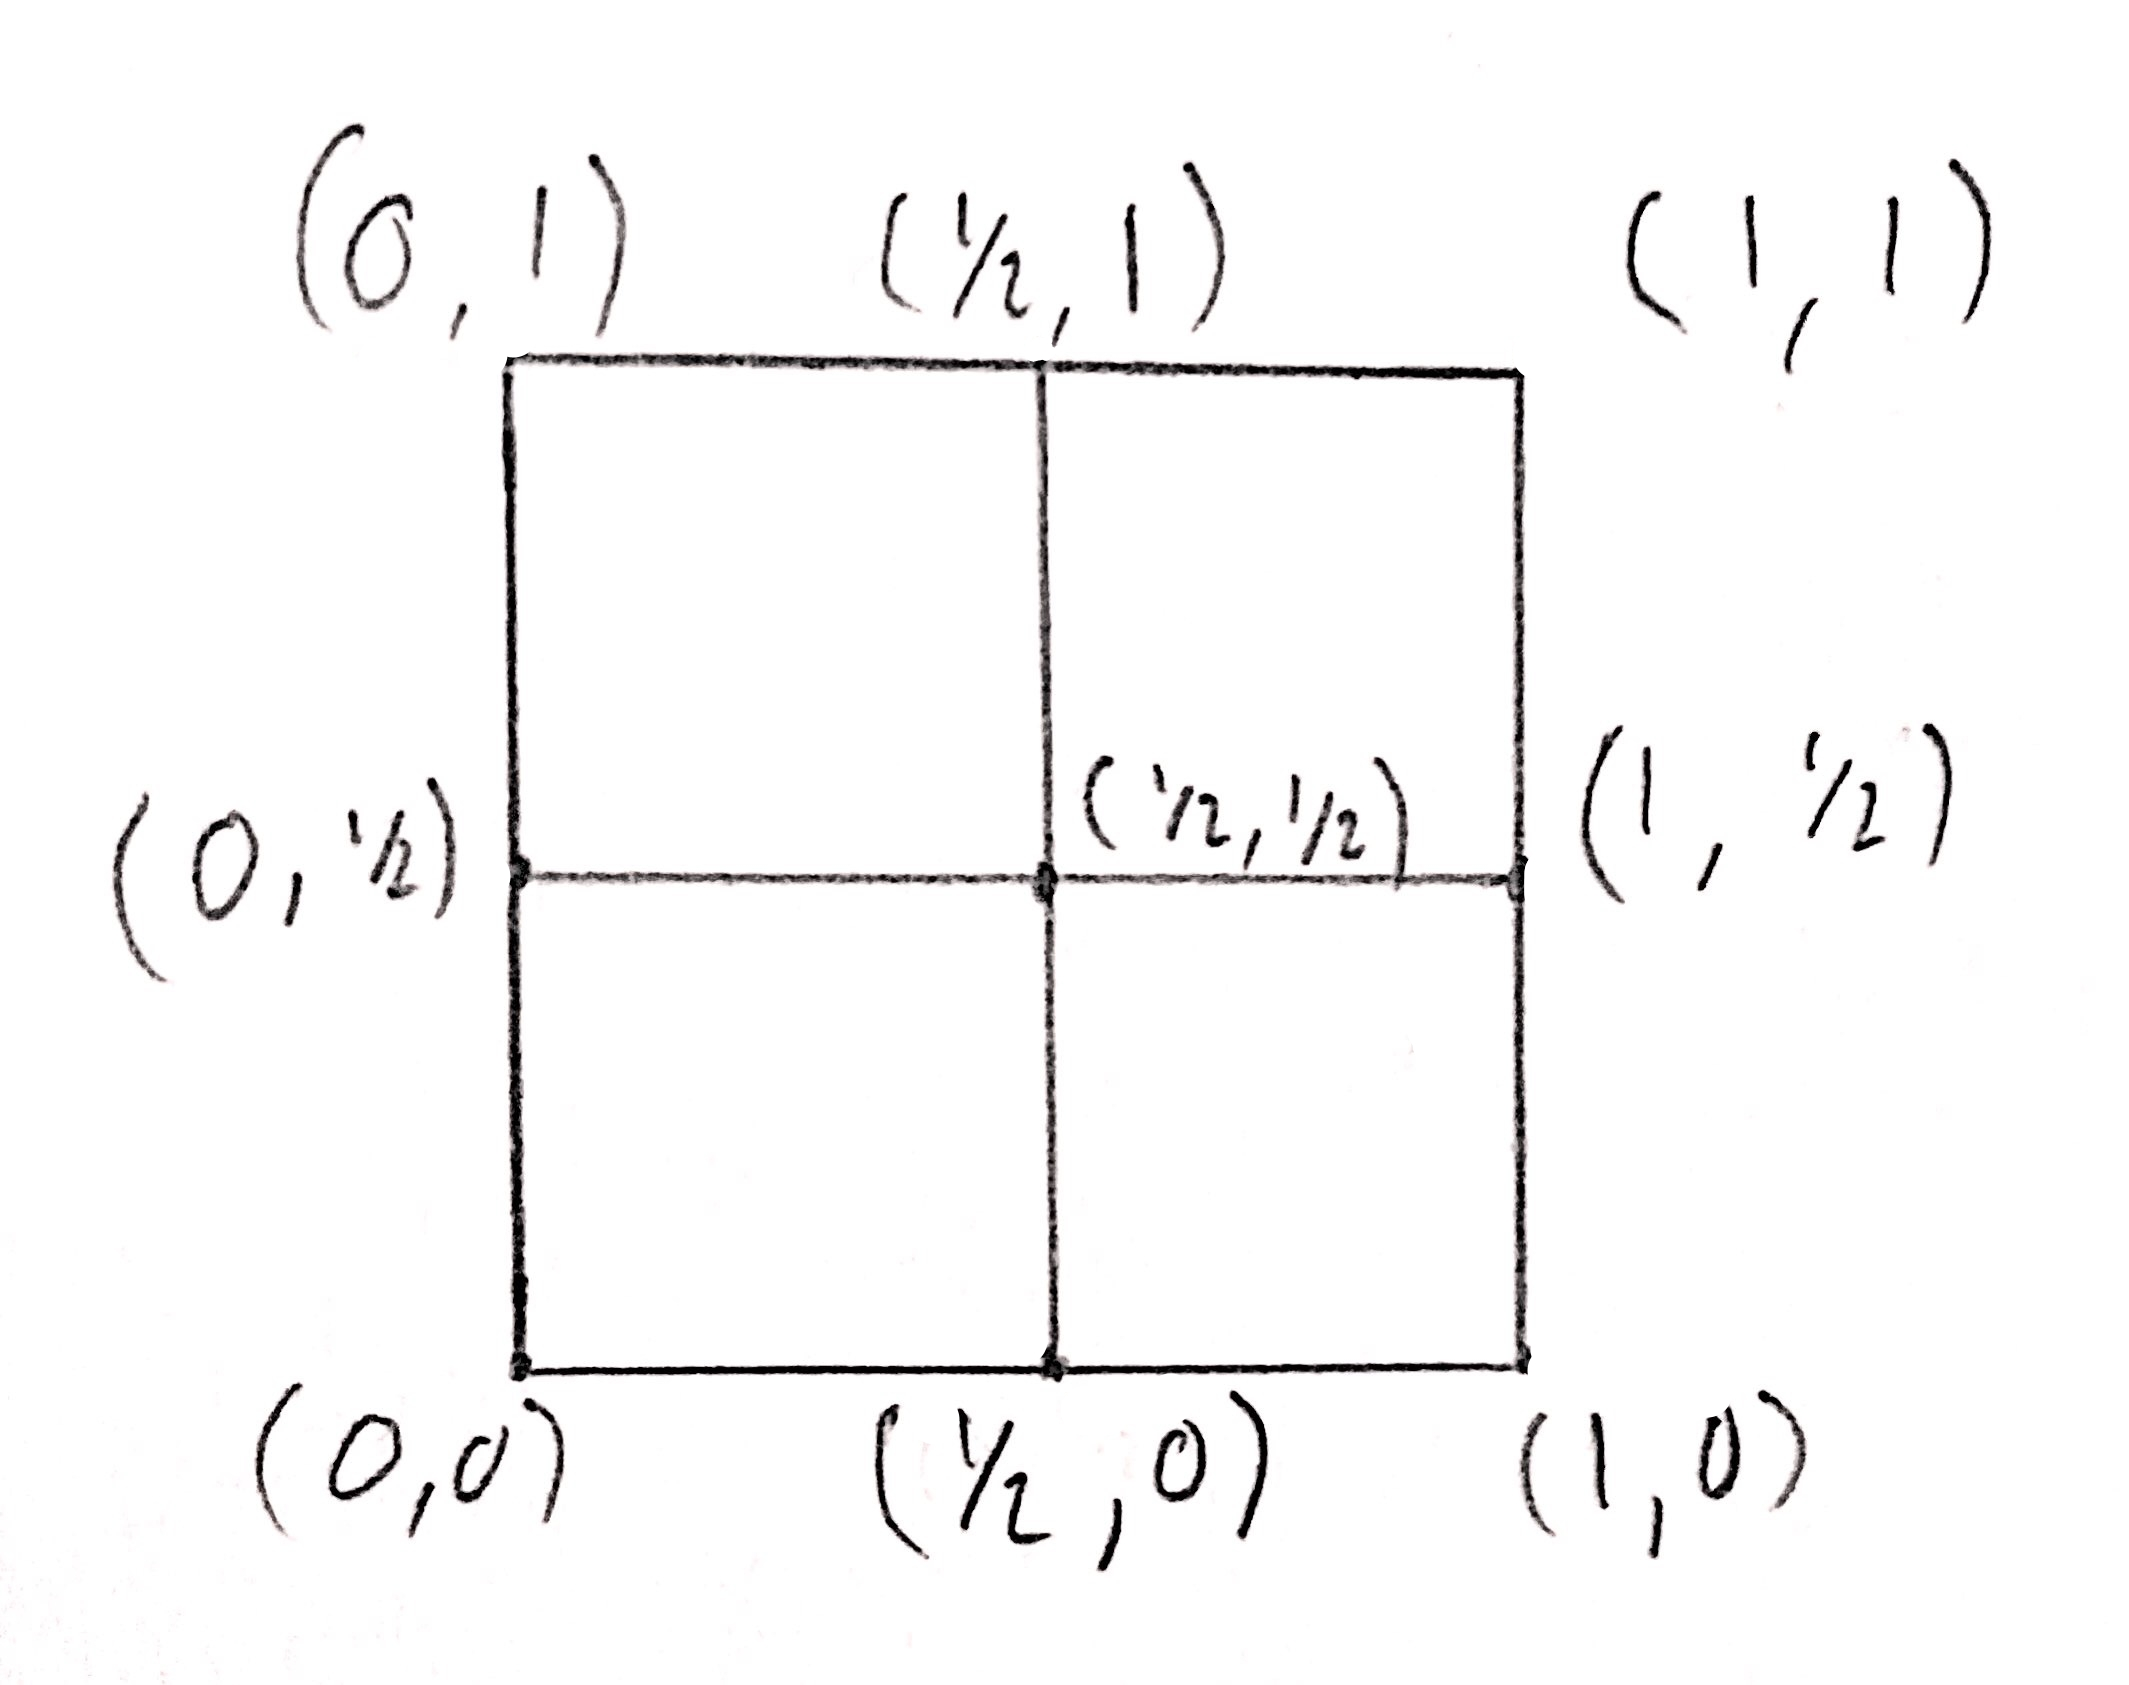
\includegraphics[scale=.06]{450b_hw8_prob1} & 
\begin{array}[b]{rcl}
L(f,P) &=&f(0,0)(\frac{1}{4})+f(\frac{1}{2},0)(\frac{1}{4})+f(0,\frac{1}{2})(\frac{1}{4})+f(\frac{1}{2},\frac{1}{2})(\frac{1}{4})\\
&=&\frac{3}{16}\\
\\
U(f,P) &=&f(\frac{1}{2},\frac{1}{2})(\frac{1}{4})+f(\frac{1}{2},1)(\frac{1}{4})+f(0,\frac{1}{2})(\frac{1}{4})+f(1,1)(\frac{1}{4})\\
&=&\frac{5}{4}\\
\\
\\
\end{array}
\end{array}
\]

\item Give an example of a rectangle $A\subset\R^n$ and functions $f$ and $g$ from $A$ to $\R$ for which $M_A(f)+M_A(g)\neq M_A(f+g)$. 

\textbf{Answer:} Let $f,g:[0,2\pi]\to\R$ be $f(x)=\sin(x)$, $g(x)=-\sin(x)$. Then 
$$M_A(f)+M_A(g) = 1+1 \neq M_A(f+g) = 0.$$


\item Let $f:\R^2\to\R$ be defined by 
\[
f(x,y)=
\begin{cases}
1 & \text{ if }x=y\\
0 & \text{ otherwise.}\\
\end{cases}
\]
Show that $f$ is integrable on $[0,1]\times[0,1]$ and find $\int_A f$. 
\begin{proof}
Observe that for any subrectangle $S=[a,b]\times[c,d]$, either $a\neq c$ or $a\neq d$, so there exists some $(x,y)\in S$ such that $f(x,y)=0$. Thus, 
$$L(f,P)=0$$ 
for any partition $P$. To show that $f$ is integrable, we will show that for any $\epsilon>0$, there exists a partition $P$ such that 
$$U(f,P)-L(f,P)=U(f,P)<\epsilon.$$

\pagebreak
Let $\epsilon>0$ be given. Choose $n\in\N$ such that
$$\tfrac{3}{n}<\epsilon.$$
Let $P_0=\{0, \frac{1}{n}, \frac{2}{n}, \dots \frac{n-1}{n}, 1\}$, and let $P=\{P_0,P_0\}$. 
\jpg{width=0.33\textwidth}{450b_hw8_prob3}
Denote $\Delta=\{(x,x)\in [0,1]\times[0,1]\}$, denote $S=\{S_i\in P : S_i\cap\Delta\neq\emptyset\}$ and $S'=P-S$. Note that $S$ contains $(3n-2)$ subrectangles, and $M_{S_i}(f)=1$ for every $S_i$. Also, $M_{S'_i}(f)=0$ for every $S'_i$ Now we calculate $U(f,P)$:
\[
\arraycolsep=1.4pt\def\arraystretch{1.5}
\begin{array}{rcl}
U(f,P) &=& \sum\limits_{i=1}^{3n-2} M_{S_i}(f)\vol(S_i)+\sum\limits_{S'} M_{S'_i}(f)\vol(S'_i)\\
&=& (3n-2)(1)(\frac{1}{n^2}) + 0\\
&<& \frac{3n}{n^2}\\
&=& \frac{3}{n}\\
&<& \epsilon. \\
\end{array}
\]

\end{proof}

\item Let $f:[0,1]\times[0,1]\to \R$ be defined by 
\[
f(x,y)=
\begin{cases}
0 & \text{if } x \text{ irrational}\\
0 & \text{if } x \text{ rational}, y \text{ irrational}\\
\sfrac{1}{q} & \text{if } x \text{ rational}, y=\sfrac{p}{q} \text{ in lowest terms.}\\
\end{cases}
\]
Show that $f$ is integrable, and $\int_{[0,1]\times[0,1]}f=0$. 
\begin{proof}
To simplify notation, let $g:[0,1]\to \R$ be defined as
\[
g(y)=
\begin{cases}
0 & \text{if } y \text{ irrational}\\
\sfrac{1}{q} & \text{if } y=\sfrac{p}{q} \text{ in lowest terms.}\\
\end{cases}
\]
Thus, 
\[
f(x,y)=
\begin{cases}
0 & \text{if } x \text{ irrational}\\
g(y) & \text{otherwise.}\\
\end{cases}
\]
We will show that:
\begin{enumerate}
\item $\sup\limits_P L(f,P)=0$.
\item [Lemma (b)] For any $\epsilon>0$, there are finitely many real numbers $y\in[0,1]$ such that $g(y)>\epsilon$. 
\item [(c)] For any $\epsilon>0$, there exists a partition $P$ such that $U(f,P)-L(f,P)<\epsilon$. 
\end{enumerate}
Thus by (a) and (c), $f$ is integrable and $\int\limits_{[0,1]^2}f=0$. 

\textbf{Proof of (a)} Observe that for any subrectangle $S=[a,b]\times[c,d]$, there exists an irrational number $\gamma$ such that $a<\gamma<b$, thus $f(\gamma, c)= m_S(f)\vol(S)=0$. Since this holds for arbitrary subrectangles, $L(f,P)=0$ for any partition $P$. \qedwhite

\textbf{Proof of Lemma (b)}. Let $\epsilon>0$ be given. For any $g(y)=\frac{1}{n}>\epsilon$, we have that $n<\frac{1}{\epsilon}$, and there are finitely many such $n\in\N$. Also, given any natural number $n$, there are finitely many fractions $\frac{k}{n}\in[0,1]$; that is, $k=1, 2, \dots, n$. Furthermore, $g\left(\frac{k}{n}\right)\geq\frac{1}{n}$ for all such fractions. Thus, $$\left\lbrace  \tfrac{k}{n} : g\left(\tfrac{k}{n}\right)\geq\epsilon, \quad k,n\in\N, \quad k\leq n\right\rbrace$$ is finite. \qedwhite


\textbf{Proof of (c)} By Lemma (b), let $\{y_1, y_2, \dots, y_n\}$ denote the rational numbers in $[0,1]$ such that
$$g(y_i)>\tfrac{\epsilon}{2}$$ 
where $i= 1,\dots, n$. Note that for $\epsilon$ smaller than 2, $y_n=1$. Let
$$\delta=\min\left\lbrace\frac{\epsilon}{4n}, \frac{\abs{0-y_1}}{2}, \frac{\abs{y_i-y_{i+1}}}{2}\right\rbrace.$$
This ensures that 
$$2\delta\leq\frac{\epsilon}{2n},$$
and that $P_y$ (defined below) is truly a partition, with terms ordered as expected. 
Let 
\[
\begin{array}{rcl}
P_x&=&\{0,1\}\\
P_y&=&\{0, (y_1-\delta), (y_1+\delta), (y_2-\delta), (y_2+\delta), \dots, (y_{n-1}-\delta), (y_{n-1}+\delta), (1-\delta), 1\},\\
\end{array}
\]
and let $P=\{P_x, P_y\}$. We denote the constituent subrectangles $S_i$ and $S'_i$ as follows:
\[
\begin{array}{rcl}
S_i &=&
\begin{cases}
[0,1]\times[(y_i-\delta), (y_i+\delta)] \phantom{\delta} & 1\leq i< n\\
[0,1]\times[(1-\delta), 1] & i=n\\
\end{cases}\\
\\
S'_i &=& 
\begin{cases}
[0,1]\times[0, (y_1-\delta)] & i=1\\
[0,1]\times[(y_{i-1}+\delta), (y_i-\delta)] & 1<i\leq n \\
\end{cases}
\end{array}
\]
\jpg{width=.33\textwidth}{450b_hw8_prob4_1}
Now, observe that 
\[
\begin{array}{rcl}
U(f,P)&=&\sum\limits_{i=1}^n M_{S_i}(f)\vol(S_i) + \sum\limits_{i=0}^n M_{S'_i}(f)\vol(S'_i)\\
%&=&\sum\limits_{i=1}^n M_{S_i}(f)(2\delta) + \sum\limits_{i=0}^n M_{S'}(f)\vol(S'_i)\\
&\leq&\sum\limits_{i=1}^n (1)2\delta + \sum\limits_{i=0}^n \frac{\epsilon}{2}\vol(S'_i)\\
&\leq&\sum\limits_{i=1}^n \frac{\epsilon}{2n} + \frac{\epsilon}{2}\sum\limits_{i=0}^n \vol(S'_i)\\
&<&\sum\limits_{i=1}^n \frac{\epsilon}{2n} + \frac{\epsilon}{2}(1)\\
&=& \frac{\epsilon}{2} + \frac{\epsilon}{2}\\
&=& \epsilon\\
\end{array}
\]
In evaluating $M_{S_i}(f)$ and $M_{S'_i}(f)$ above, we used the fact that $f$ is bounded above by 1, and the fact that every $y_i$ such that $g(y_i)>\frac{\epsilon}{2}$ is contained in exactly one $S_i$. Thus, $M_{S_i}(f)\leq 1$ and $M_{S'}(f)\leq \frac{\epsilon}{2}$ for all appropriate $i$. 

Therefore, given any $\epsilon>0$, we have produced a partition $P$ such that $U(f,P)-L(f,P)<\epsilon$, so we are done. 
\end{proof}

\item 
\begin{enumerate}
\item Let $A\subset \R^n$ be a rectangle, and assume that $f:A\to\R$ is integrable and satisfies $F\geq 0$ on $A$. Prove that $\int_A f\geq0$. 
\begin{proof}
For any subrectangle $S$ of any partition $P$ of the domain $A$, 

\begin{tabular}{rl}
$f(\vecb{x})\geq0$ &for any $\vecb{x}\in S$, so \\
$m_S(f)\geq0$ &for any $S\in P$, so \\
$L(f,P)\geq0$ &for any partition $P$ of $A$, so \\
\end{tabular}

since $0\leq L(f,P)\leq\int_A f$, then we are done. 
\end{proof}
\item Assume in addition that $f$ is continuous and $f$ is positive at some point in $A$. Prove that $\int_A f>0$. 
\begin{proof}
Let $a$ denote the assumed element of $A$ such that $f(a)>0$. Let $\epsilon=f(a)$. Since $f$ is continuous, there exists some $\delta>0$ such that if $x\in A$ and $\norm{x-a}<\delta$, then $\abs{f(x)-f(a)}<\epsilon$, so $f(x)>0$. Now, let $P$ be a partition of $A$ containing the subrectangle 
$$S_0=\prod_{i=1}^n\left[\left(a_i-\tfrac{\delta}{\sqrt{n}}\right),\left(a_i+\tfrac{\delta}{\sqrt{n}}\right)\right].$$
Since $S_0\subset B(a,\delta)$, 
$$m_{S_0}(f)>0,$$
and by (a), $$m_S(f)\geq0$$ for all other $S$, so $$L(f,P)<\int_A f$$ and we are done. 
\end{proof}
\end{enumerate}


\end{enumerate}
\end{document}
